\clearpage
%//==============================--@--==============================//%
\subsection[3.3 Connectionless Transport: UDP]{\hspace*{0.075 em}\raisebox{0.2 em}{$\pmb{\drsh}$} Connectionless Transport: UDP}
\label{subsec:UDP}

\noindent \textbf{Nota:} As sockets UDP são identificada somente por dois campos: porto de destino e endereço IP de destino. Tal significa que informação oriunda de dois \textit{hosts} diferentes (consequentemente IP's de origem diferentes) cujos destinos possuem o mesmo IP e o mesmo porto será recebida pela mesma \textit{socket}.

\vspace{1 em}
\noindent A estrutura de um segmento UDP é a seguinte:

\begin{figure}[H]
    \centering
    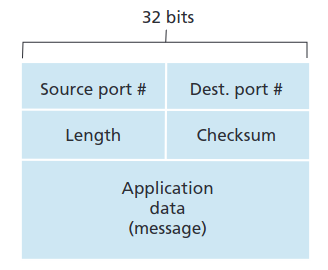
\includegraphics[width = 0.5\linewidth]{img/3/UDP-segment.png}
    \caption{Estrutura de um segmento UDP}
    \label{fig:seg-UDP}
\end{figure}

\begin{itemize}
    \item The UDP header has only four fields, each consisting of two bytes.
    \item The port numbers allow the destination host to pass the application data to the correct process running on the destination end system (that is, to perform the demultiplexing function).
    \item The length field specifies the number of bytes in the UDP segment (header plus data). An explicit length value is needed since the size of the data field may differ from one UDP segment to the next.
    \item The checksum is used by the receiving host to check whether errors have been introduced into the segment (como já referido, o protocolo garante apenas deteção de erros).
\end{itemize} 

%//==============================--@--==============================//%
\subsubsection[3.3.1 Checksum]{$\pmb{\rightarrow}$ Checksum}
\label{subsubsec:checksum}

\begin{mdframed}
    \begin{center}
        \textbf{Checksum (soma de verificação):} $\overline{x_1 \oplus \dots \oplus x_m} = 2^n - 1 - \left(x_1 \oplus \dots \oplus x_m \right)$
    \end{center}
    \vspace{-0.5em}
    \begin{quote}
        ``$[$The$]$ Sender side performs the 1s complement of the sum of all the 16-bit words in the segment"\cite{Kurose2017}
    \end{quote}
\end{mdframed}

\begin{quote}
    ``The UDP checksum provides for error detection. That is, \textbf{the checksum is used to determine whether bits within the UDP segment have been altered} (for example, by noise in the links or while stored in a router) as it moved from source to destination."\cite{Kurose2017}
\end{quote}

\noindent \underline{\textbf{Relembrar}}: Soma binária com \textit{wrapping} em caso de \textit{overflow}
$$
    x \oplus y = 
    \begin{cases}
        x + y, & x + y < 2^n \\
        x + y - 2^n + 1, &  x + y \ge 2^n
    \end{cases}
$$

\newpage
\noindent \textbf{Exemplo:} Supondo um segmento composto por 3 palavras de 16 bits. 

\begin{center}\texttt{%
    0110011001100000 \\
    0101010101010101 \\
    1000111100001100
    }
\end{center}

\begin{figure}[H]
    \centering
    \begin{minipage}{0.45\linewidth}%
        \begin{center}
        The sum of first two words is: \\[6pt]
        
        \texttt{%
            0110011001100000 \\
            0101010101010101 \\
            ------------------------------- \\
            1011101110110101
        }
        \end{center}
    \end{minipage}
    \raisebox{0.25em}{$\pmb{\rightarrow}$}
    \begin{minipage}{0.45\linewidth}%
        \begin{center}
        Adding the third word gives: \\[6pt]
        
        \texttt{%
            1011101110110101 \\
            1000111100001100 \\
            ------------------------------- \\
            0100101011000010
        }
        \end{center}
    \end{minipage}
    \label{fig:checksum}
\end{figure}

\vspace{-1.25
em}
$$
   \pmb{\therefore} \text{The 1s complement of the sum \texttt{0100101011000010} is \underline{\texttt{1011010100111101}}}
$$

\noindent Lastly, ``At the \textbf{receiver}, all \underline{four} 16-bit words are added $[$the segment's words and the checksum$]$. If no errors are introduced into the packet, then clearly the sum at the receiver will be \texttt{1111111111111111}."\cite{Kurose2017}

\vspace{0.75em}
\noindent \textbf{Nota:} Neste exemplo, a ultima soma resulta num \textit{overflow} que sofre um \textit{wrap around}, i.e., o bit de excesso é somado ao bit menos significativo do resultado. 
%//==============================--@--==============================//%